\begin{thm}{149}{\hosi 5\maru}{京大オープン (2016)}
 $p$は正の定数とする。$xy$平面上の2曲線、
 \begin{align*}
  C_1:\quad & |y|=\tan x \quad (0\le x < \frac{\pi}{2}) \\
  C_2:\quad & x=\frac{y^2}{4}+p
 \end{align*}
 が2点で接しているとする。$C_1$と$C_2$で囲まれた部分の面積を求めよ。
\end{thm}

2つの曲線はともに$x$軸について対称であるから、$y\ge 0$についてのみ考えれば十分。よって$C_1$は代わりに$y=\tan x$~$\left(0\le x< \dfrac{pi}{2}\right)$を考え、$C_2$は$y=2\sqrt{x-p}$を考える。$C_2$は$x\ge p$の範囲にある曲線なので、$C_2$と共有点を持つためには$p<\dfrac{\pi}{2}$であることが必要である。また、$p>0$であるから$\tan p>0$であり、一方$C_2$では$x=p$のとき$y=0$であるから、$x=p$なる点では2曲線が接することはない。

接点の$x$座標を$t$とするとき、$p<t<\dfrac{\pi}{2}$である。接点の$y$座標が等しくなるから、$\tan t=2\sqrt{t-p}$である。また接線の傾きも等しくなる。$C_1$については、$y'=\dfrac{1}{\cos^2 x}$である。$C_2$については、$y'=\dfrac{1}{\sqrt{x-p}}$である。したがって、$\dfrac{1}{\cos^2 t}=\dfrac{1}{\sqrt{t-p}}$である。以上によって、$t$と$p$について、
\begin{align*}
 \left\{
 \begin{aligned}
  \tan t&=2\sqrt{t-p} \\
  \frac{1}{\cos^2 t}&=\frac{1}{\sqrt{t-p}}
 \end{aligned} \right.
\end{align*}
の連立方程式を得る。$\sqrt{t-p}=u$とおき、$\dfrac{1}{\cos^2 t}=1+\tan^2 t=1+4u^2$を下式に代入すれば、
\[ 1+4u^2=\frac{1}{u} \,\dou\, 4u^3+u^1=0 \,\dou\, (2u-1)(2u^2+u+1)=0 \]
という$u$についての方程式を得る。明らかに$u>0$より、$u=\dfrac{1}{2}$と求まる。したがって、$t=p+\dfrac{1}{4}$を得る。上式から$\tan t=1$となるから、$t=\dfrac{\pi}{4}$とわかる。また$p=\dfrac{\pi-1}{4}$。

\begin{wrapfigure}[10]{r}[0pt]{100pt}
 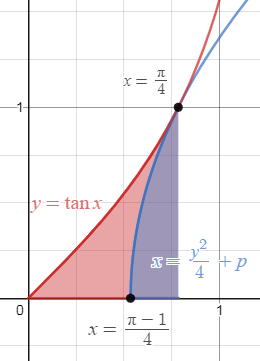
\includegraphics[width=\linewidth]{../problems/Q_149/A_149.png}
\end{wrapfigure}
以上より、$y\ge 0$における$C_1$, $C_2$のグラフは右図のようになる。$C_1$, $C_2$と$y=0$で囲まれた部分の面積を、赤部とから青部を引くことによって求める。
\begin{align*}
 & \int_0^t\! \tan x \,dx -\int_p^t\! 2\sqrt{x-p} \,dx \\
 =& \Bigl[-\log\cos x\Bigr]_0^t - \Bigl[\frac{4}{3}(x-p)^{\frac{3}{2}}\Bigr]_p^t \\
 =& \log\cos\frac{\pi}{4}-\frac{4}{3}u^3 = \frac{\log2}{2}-\frac{1}{6}
\end{align*}
これの2倍が求める面積であるから、$\log 2-\dfrac{1}{3}$